\chapter{移动机器人导航技术及相关知识}

\section{引言}
当今,移动机器人已经广泛应用于自动化物流、仓储管理、医院和办公室等领域
,使得人们的工作更加高效和便利。导航系统是移动机器人的关键功能模块,
移动机器人导航技术是指通过多种传感器获取环境信息,对机器人的位置、速度、
方向等状态进行估计和控制,以实现机器人自主移动的过程。其输入信息包括机器
人当前位置、目标位置、环境地图、障碍物等,输出信息包括机器人运动的速度、
方向、路径等。移动机器人导航系统是一个复杂的耦合系统,同时移动机器人导航
技术也是一个多学科的交叉技术。本章节主要探究移动机器人导航系统中所涉及到
的关键技术,将组成导航系统的各个关键模块之间的关系和为导航系统提供的功能
详细解读以及展示这些关键技术在目前产品以及demo模型中的应用。由于导航技术
牵扯较多,故本章以导航中各模块涉及到的技术领域为章节,详细展开。

\section{移动机器人导航概述}
移动机器人导航系统是一个复杂的多元系统,主要是通过传感器,例如激光雷达感知
环境,同时对自身位置进行定位,在构建的全局先验地图基础上进行路径规划,期间
局部规划并且避障,将控制信号交给执行部件,完成移动过程。
其中涉及到多个学科门类,在最基础的导航任务中,所需要的相关知识主要有如下
几个方面:

1.传感器技术移动机器人的导航需要依靠传感器技术,例如激光雷达、摄像头、
超声波传感器等。这些传感器可以帮助机器人感知周围环境,识别障碍物和地标,
并提供机器人的位置和方向信息。

2.地图建模在移动机器人导航系统中,地图建模是非常重要的环节。地图建模的
主要任务是将机器人所在的环境转换成机器人可识别的数字化地图。数字化地图
通常包括地图边界、地形高度、障碍物位置和机器人目标位置等信息。常用的地
图建模方法包括激光雷达扫描、视觉SLAM(Simultaneous Localization and Mapping)等。

3.定位模块,在地图建模的基础上,移动机器人需要掌握自身处于环境中的位姿,
定位的精准程度直接影响到移动机器人规划和执行的效果。定位的信息包括机器人
目前处于建模后环境的位置以及坐标系位姿等。最常见的定位方法有SLAM方法、
卫星定位系统。

3.路径规划在数字化地图上,机器人需要能够规划出一条合适的路径以达到目的
地。路径规划的方法通常是基于机器人的位置和目标位置,利用搜索算法、最短
路径算法等方法来生成一条合适的路径。其中,常见的路径规划算法包括A*算法
、Dijkstra算法、RRT(Rapidly-exploring Random Tree)算法等。

4.运动控制机器人在移动时需要控制轮子或足部运动,以使其沿着规划好的路径
行进。运动控制的目标是实现机器人的准确定位、平稳移动和灵活转向。运动控
制方法包括PID控制、模糊控制等。

5.局部避障在移动过程中,机器人需要避开障碍物,这就需要局部避障算法。常
见的局部避障算法包括基于代价地图的避障方法、局部避障算法等。

6.实现和测试
最后,将以上技术组合起来,实现一个完整的移动机器人导航系统,并进行测试
和优化。测试的方法包括模拟测试和实际场地测试。在模拟测试中,可以使用虚
拟仿真软件模拟机器人在不同环境下的导航情况。而在实际场地测试中,需要在
实际环境中测试机器人的导航性能,如准确定位、路径规划、避障等方面的表现
。测试结果可以用来优化算法和调整系统参数,以提高机器人导航的准确性和效
率。
总之,移动机器人导航系统的实现需要从传感器技术、地图建模、路径规划、运
动控制、局部避障等多个方面进行综合考虑和设计,才能实现一个稳定、可靠、
高效的自主导航系统。


其任务示意图可以表示如下:

\begin{figure}[ht]
    \centering
    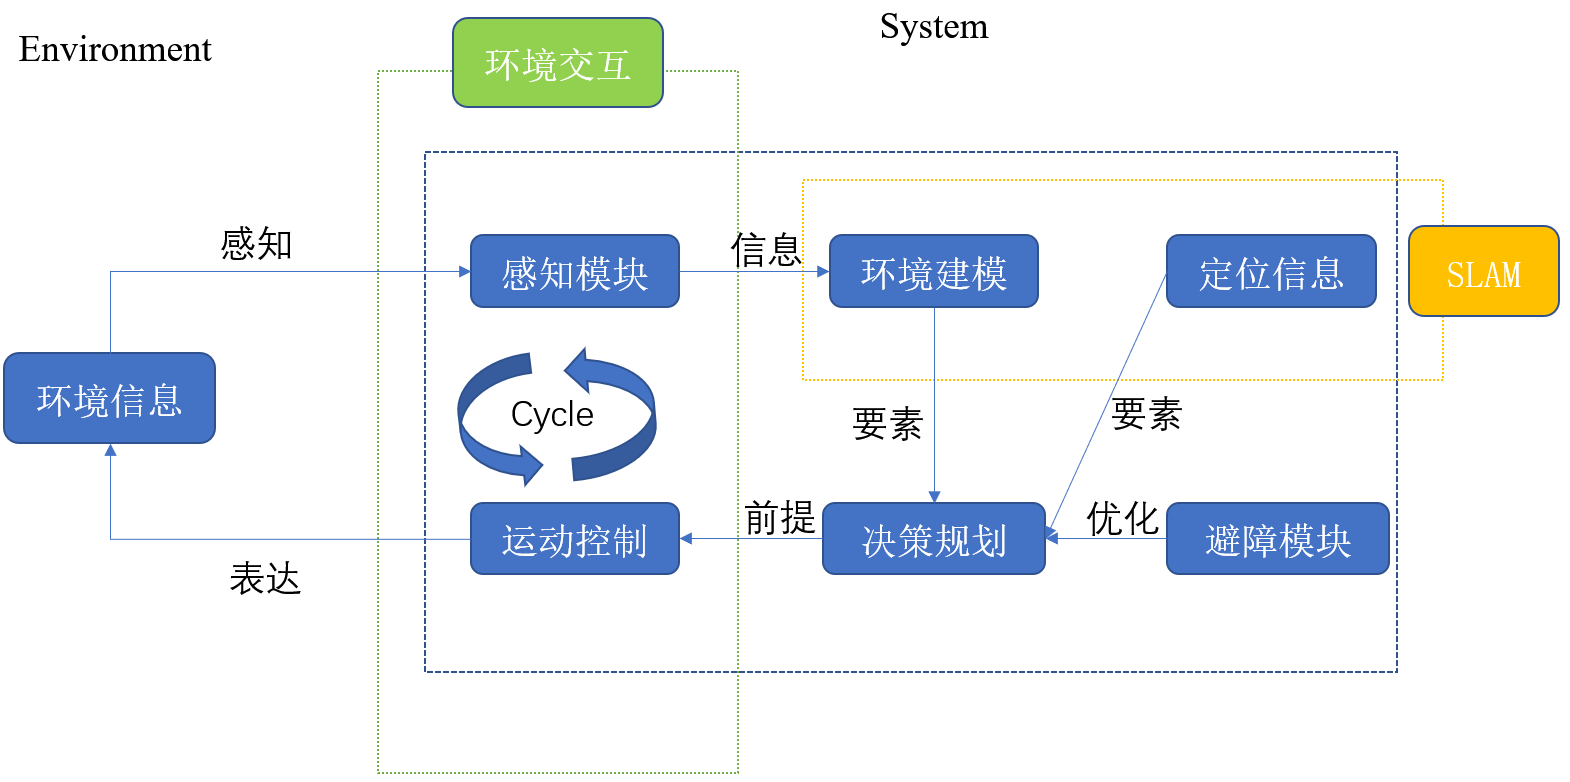
\includegraphics[scale=0.42]{navi_task.png}
    \caption{导航任务示意图}
\end{figure}
图中,感知模块和运动控制是与环境进行交互的模块,在交互过程中不断循环,通
过感知模块摄取环境信息,并通过运动控制模块执行表达,体现为在环境中的行为;
在导航系统内部,通过感知模块感知到的信息,对环境进行建模,为决策规划提供
要素,没有环境信息的导航系统无法执行有效决策规划;决策规划同时需要定位信
息作为要素一部分,导航系统了解自身在建模的环境中的位置之后便具有决策规划
的能力;但导航系统的前提是要安全,那么需要避障模块对决策规划结果进行优化,
得到无碰撞的规划信息,此信息最终转换成运动控制信号,由具体执行部件,例如
电机、车轮等执行,表达为在环境中的行为。

其中环境建模与定位信息可以通过独立模块运行工作,也可以通过SLAM(Simultaneous Localization and Mapping)
技术提供实时的定位建图。但在园区的全局地图下,为保证系统稳定,多采用单独建
图、后期处理的方式取得质量较高的地图;并通过GPS全球定位系统等方式进行定位
或者辅助定位,具体取决于精度要求。


\section{感知模块技术基础}
感知模块的基础是各种各样的传感器,目前广泛应用于移动机器人行业的传感器主要
两种:激光雷达和相机。

\subsection{激光雷达}
激光雷达(LIDAR)是一种主动式传感器,通过向周围环境发射激光束,并通过接收
反射回来的激光束来获取环境的深度和距离信息,能够提供高精度、高分辨率的环
境信息。激光雷达的内部组成主要有以下器件:

1.激光器:激光雷达使用的激光器需要具有高功率和短脉冲宽度,以实现高精度的
测量。一般采用半导体激光器或固体激光器。
半导体激光器:半导体激光器是一种基于半导体材料的激光器,通常采用GaN、InG
aN等III-V族化合物半导体材料,具有小体积、低功耗、长寿命、易于集成等优点。
半导体激光器的输出波长范围一般在400~1700nm之间,适用于大部分激光雷达应用。
固体激光器:固体激光器是一种基于晶体或玻璃材料的激光器,通常采用Nd:YAG、
Er:YAG等材料,具有高功率、高效率、高稳定性等优点。固体激光器的输出波长范
围一般在1000-1500nm之间,适用于长距离和低散射噪声的应用。

2.接收器:接收器是用于接收反射回来的激光束的组件。一般采用光电二极管(pho
todiode)或光电探测器(photodetector)。
光电二极管:光电二极管是一种将光转化为电信号的半导体器件,具有响应速度快、
灵敏度高、体积小、成本低等优点。光电二极管的工作原理是当光照射到P-N结上时,
会产生电子-空穴对,从而产生电流信号。
光电探测器:光电探测器是一种将光转化为电信号的器件,包括光电二极管、光电
倍增管、光电导管等。光电探测器的响应速度和灵敏度较高,适用于激光雷达等高
精度应用。

3.光学器件:激光雷达使用的光学器件包括镜头、光栅和棱镜等。它们的作用是对激光束进行聚焦、分束、旋转等操作。
镜头:镜头是一种用于聚焦光线的光学器件,通常用于激光雷达中的发射器和接收
器。激光雷达发射器需要将激光束聚焦成尽可能小的直径,以便实现高精度的距离
测量。接收器则需要将反射回来的光线聚焦在光电探测器上,以提高接收效率和精度。

4. 旋转平台:旋转平台是激光雷达中常见的机械部件,可以使激光雷达以一定的速
度和角度旋转,以获取360度的空间信息。旋转平台通常采用步进电机或直流电机驱
动,可实现高精度的旋转控制和稳定性。

5.距离测量算法:激光雷达通过测量激光束的往返时间和波长,可以计算出目标物
体到激光雷达的距离。常见的距离测量算法包括TOF(Time of Flight)和FMCW(
Frequency Modulated Continuous Wave)。
TOF算法:即飞行时间测量(Time of Flight)算法,是一种基于激光脉冲往返时间
的距离测量算法。其基本原理是通过测量激光束从激光雷达发射出去后反射回来所需
的时间来计算物体与激光雷达之间的距离。
当激光束从激光雷达发射出去时,它会在空气中以光速c传播。当激光束遇到一个物
体时,它的能量将部分地被吸收并转换为热能,同时一部分激光能量将反射回激光雷
达。反射激光的时间和激光束的传播速度是已知的,因此可以通过这些信息计算物体
的距离。
如下图所示,当激光束射向目标物体时,激光雷达记录下发射时间t1和反射时间t2。
\begin{figure}[ht]
    \centering
    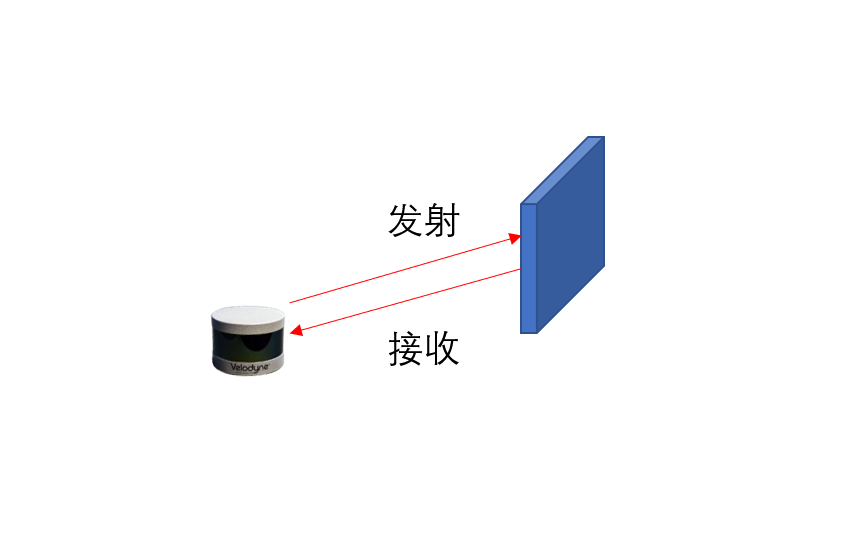
\includegraphics[scale=0.5]{ToF.png}
    \caption{基于ToF原理的激光雷达测距示意图}
\end{figure}
物体到激光雷达的距离R可以通过下式计算得到:
\begin{equation}
    L = c(t_2 - t_1) / 2
\end{equation}

其中,c是光速,t1和t2是激光束发射和反射的时间差。TOF算法的优点是测量精度高、
测量速度快、简单、成本低,但其测量精度受到环境光、物体表面反射率等因素的影响。


FMCW算法:即调频连续波(Frequency Modulated Continuous Wave)算法,是一种
利用激光频率变化来测量距离和速度的方法。在FMCW激光雷达中,激光束通过一个运
动的镜片反射,产生频率偏移。当激光束与物体相交时,反射激光会随着物体的运动
而产生频率偏移。
FMCW激光雷达通过改变激光的频率来实现距离和速度的测量。激光雷达发射一个连续
的线性调频激光波,即下行斜坡。当激光束照射到物体上时,部分激光会反射回来,
这部分反射激光的频率会与下行斜坡的频率有所不同。接着,激光雷达发射上行斜坡,
这时反射激光会与上行斜坡产生干涉,形成一个频率等于反射激光频率与上行斜坡频
率之差的混频信号。接下来,通过对混频信号进行FFT变换,可以得到频谱图。频谱
图中的峰值对应着物体反射激光的频率,因此可以通过这些信息来计算物体与激光雷
达之间的距离。
FMCW算法的优点是精度高、抗干扰能力强,可以同时测量距离和速度,但成本较高。

\subsection{摄像头}
摄像头是一种基于视觉感知的设备,它可以将物体的图像转换成数字信号进行处理。
与激光雷达不同,摄像头通过感知光的反射来获取环境中的信息。摄像头通常由透
镜、图像传感器和信号处理器等组成。

1.透镜:摄像头的透镜通常由多个光学镜片组成,其作用是将环境中的光线聚焦到
图像传感器上。

2.图像传感器:通常有两种类型:CCD(Charged Coupled Device)和CMOS(Comp
lementary Metal-Oxide-Semiconductor)。CCD传感器是传统的图像传感器,通
过在晶体管阵列中收集和移动电荷来捕获图像。而CMOS传感器则是现代摄像头常用
的传感器类型,它将光电转换器集成在每个像素中,可以通过集成其他功能来实现
更高级的图像处理和计算任务。近年来,CMOS传感器因其成本低、功耗低和性能高
而逐渐取代了CCD传感器,成为现代摄像头的主流传感器类型。

3.信号处理器:将得到的电子信息转换为数字信号,以形成数字图像或视频,通常由
多个阶段组成,包括预处理、增益控制、降噪和色彩校正等。这些步骤旨在提高图像
的质量和清晰度,并消除图像中的噪声和失真。

摄像头的性能主要由分辨率、帧率、动态范围、色彩深度和信噪比等指标来衡量。
分辨率指图像中的像素数量,通常用宽×高来表示。帧率是指摄像头每秒输出的图
像数量,通常用赫兹来表示。动态范围是指摄像头能够捕捉到的最大和最小光强之
间的范围。色彩深度是指每个像素可以表示的颜色数。信噪比是指信号和噪声之间
的比例,它越高则图像的质量越好。

\section{环境建模}
在移动机器人导航领域中,机器人需要一个可供内部系统识别的环境模型,此模型
需要能够表达环境的特征信息,例如位置距离和物体结构等。
环境建模的方式有很多种,例如:
点云地图(Point Cloud Map)、栅格地图(Grid Map)、拓扑地图(Topological Map)

三维网格地图(3D Grid Map):将环境划分为三维网格,将每个网格的状态(如
障碍物、自由空间等)作为该网格的属性进行存储。与栅格地图类似,但能够更加
准确地表示环境中的物体形状和位置。
深度图(Depth Map):使用深度传感器(如激光雷达、RGB-D相机等)获取环境中
物体的深度信息,并将其表示为灰度图或RGB图像。适用于需要进行三维重建或深度
感知的任务。
语义地图(Semantic Map):将环境中的物体按照其语义类别进行分类和建模,并
将其位置、大小、形状等信息保存为语义地图。适用于需要进行高级任务规划、交
互和理解的任务。
光流场(Optical Flow Field):使用光流算法从视频流中提取物体在图像中的
运动信息,并将其表示为光流场。适用于需要进行移动物体追踪、目标检测和位姿
估计的任务。
轨迹(Trajectory):记录机器人或其他物体的运动轨迹,并将其表示为一系列
位置坐标和时间戳的数据。适用于需要进行轨迹分析、路径规划和行为分析的任务。
场景图(Scene Graph):将环境中的物体表示为图的节点,将它们之间的关系(
如包含、连接、属性等)表示为图的边。适用于需要进行场景理解、关系推理和知
识表示的任务。
移动机器人领域最常使用的环境建模方式,主要有点云地图、栅格地图和拓扑地图。

\subsection{点云地图}
点云地图将环境中的物体和障碍物的位置、形状等信息保存为点云数据,是一种基
于几何形状的建模方式。点云地图适用于需要高精度的环境建模和精确的感知任务,比如自动驾驶、机器人导航等。

在SLAM技术未有突破前,卫星定位系统和激光雷达等传感器采集数据后期建图的方式是主流,此种方式耗时较高,但是建图精度高,可以后期人工纠偏,如今许多园区的高精度地图仍然使用此类方法。

目前更多的在非园区场景下使用基于SLAM方法的同步建图方式,该方式建图速度快,成本低廉,例如\citet{zhang2014loam} 提出了一文提出了一种实时的激光雷达点云地图构建算法。该算法通过在点云中提取特征点,并基于特征点之间的关系进行位姿估计和运动估计,实现了高效的点云地图构建。在其改进版本LeGO-LOAM中,\citet{shan2018lego}将点云数据分为地面点和非地面点两类,并在地面点的处理中引入了高斯混合模型(Gaussian Mixture Model, GMM)对地面点进行建模。通过对地面点进行建模,可以减少环境中非地面点对定位和地图构建的干扰,进一步提高算法的精度和鲁棒性。\citet{wan2018robust}涉及到了点云地图构建的问题。该方法通过多传感器融合,将激光雷达数据和摄像头数据进行融合,生成高精度的三维地图,从而实现车辆在复杂城市环境中的高精度定位和导航。
如图是LOAM所建的点云地图:

\begin{figure}[ht]
    \centering
    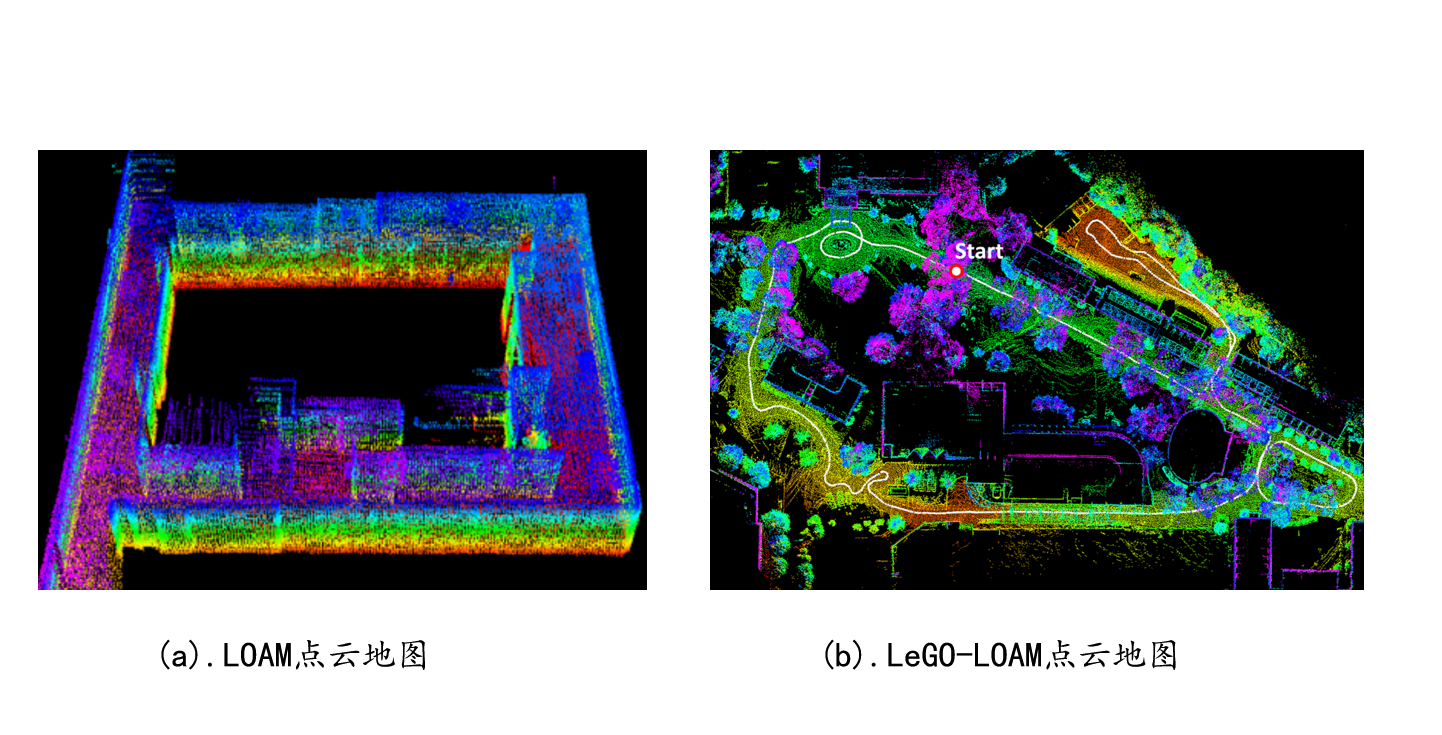
\includegraphics[scale=0.46]{loams.png}
    \caption{LOAM簇算法所建点云地图}
\end{figure}

\subsection{栅格地图}
栅格地图将环境划分为网格,将每个网格的状态(如障碍物、自由空间等)作为该网格的属性进行存储,是一种基于空间状态的建模方式。栅格地图适用于需要快速生成环境模型和实时感知任务,比如移动机器人、无人机等。栅格地图中的占据状态通常由二值化的栅格单元格表示,其中
栅格地图的内部占用概率投票方式\cite{durrant2006simultaneous}为:
\begin{equation}
P(m_i | z_{1:t}, x_{1:t}) = \frac{1}{1 + e^{-l_i}}
\end{equation}
其中 $m_i$ 表示第 $i$ 个栅格单元格的占据状态, $z_{1:t}$ 表示前 $t$ 个时刻的所有观测值, $x_{1:t}$ 表示前 $t$ 个时刻机器人的所有位姿, $l_i$ 表示单元格 $i$ 的 log-odds 值,其计算方式为:

\begin{equation}
l_i = \log \frac{P(m_i = 1 | z_{1:t}, x_{1:t})}{P(m_i = 0 | z_{1:t}, x_{1:t})}
\end{equation}

在实际应用中,栅格地图的占据状态投票概率可以使用不同的方法来计算和更新,例如最大似然法、贝叶斯法、递归贝叶斯法等。最终目的就是对栅格单元格进行占据状态的评估,以进行后续的在栅格地图上的路径规划和避障等任务。
移动机器人在栅格地图中的位置具体表现由当前所使用的规划算法决定,例如在A*算法\cite{hart1968formal}的规划任务中,栅格地图上移动机器人的位置以向量形式表示,例如(x, y , z),但若使用考虑机器人运动学模型约束的算法Hybrid A*\cite{likhachev2008planning},则拥有机器人运动学模型约束的移动机器人位姿通常以(x, y, $\theta$ )表示,其中$\theta$ 表时当前机器人的位置朝向。

\subsection{拓扑地图}
拓扑将环境中的物体和障碍物抽象为节点,将它们之间的关系(如连接关系、距离等)作为图的属性进行存储,是一种基于拓扑关系的建模方式。拓扑地图适用于需要高层次的环境表示和规划任务,比如园区与城市地图上的任务规划等。
拓扑地图的构建过程主要是提取地标、建立节点、建立拓扑关系。提取地标的过程就是筛选节点的过程,而后建立相应的节点(node),在节点之间,根据两节点之间的可通行性,判断两节点之间是否有边(edge),若有边,则互相联通。这也称为建立拓扑关系的过程,建立拓扑关系:根据节点之间的空间关系建立拓扑关系。这些关系可以是直接测量的距离或角度,也可以是通过机器学习方法推断得出的。建立拓扑关系的方法有很多种,其中一种常用的方法是使用基于距离的方法,如Voronoi图。基于距离的方法将空间分成不同的区域,每个区域都对应一个节点。然后,使用距离信息将这些节点相连,建立拓扑关系。另一种方法是基于相邻性的方法,如最近邻算法或RANSAC算法。
拓扑地图相对于栅格地图和点云地图相比,1.可扩展性强:拓扑地图中的节点和边缘可以随时添加或删除,而不需要对整个地图进行重新构建。因此,拓扑地图能够更好地应对环境的变化。
2.可解释性强:拓扑地图中的节点和边缘通常具有语义信息,能够描述环境中的重要位置和关系。因此,拓扑地图能够提供对环境更深入的理解。
3.更高的效率:由于拓扑地图通常是稀疏的,路径规划和定位等算法可以更快速地执行。
4.更少的数据存储:与其他地图形式相比,拓扑地图通常需要存储的数据更少,因为它们只包含有用的拓扑信息。
5.鲁棒性强:拓扑地图中的节点和边缘可以使用不同的噪声滤波器进行平滑和处理,从而提高了定位和规划的鲁棒性。
因此,拓扑地图在大型的高层次环境表达和路径规划领域,具有相当广泛的应用,同时,RRT\cite{lavalle1998rapidly}、RRT*\cite{karaman2011sampling}以及其它衍生规划算法与拓扑地图具有极高的适配性。
\section{决策规划}
决策规划部分可以根据实际应用中所属的层次分为局部规划和全局规划方法。

\subsection{局部规划}
人工势场法:
人工势场法是一种基于势场的局部路径规划方法,它通过在机器人周围建立势场,使得机器人沿着势场梯度的方向移动。人工势场法的优点是简单易实现,实时性好,但容易出现局部最小值陷阱问题。
人工势场法的基本思想是将机器人和障碍物看作是带电荷的物体,机器人之间相互排斥,机器人与障碍物之间相互吸引。机器人在势场中的移动方向是势场梯度的方向,即向势能下降最快的方向移动。

滑动窗口法:
滑动窗口法是一种基于轨迹的局部路径规划方法,它将机器人的轨迹分为若干个滑动窗口,然后在每个滑动窗口内进行规划。滑动窗口法的优点是可以在不同的窗口内采用不同的路径规划算法,能够更好地适应不同的环境。
滑动窗口法的基本思想是在机器人当前位置和目标位置之间建立一系列重叠的滑动窗口,通过窗口内的路径规划得到机器人的局部路径,然后将不同窗口内的路径拼接起来得到机器人的全局路径。


\subsection{全局规划}
全局规划算法分为启发式算法和人工智能算法。
\subsubsection{启发式算法}
Dijkstra 算法:
Dijkstra 算法由 E.W. Dijkstra 在 1959 年提出。 它是解决有向图中最短路径问题的典型最短路径算法。 它的主要特点是以起点为中心延伸到终点。 图的每条边由两个顶点组成一个有序元素对。 边的值由权重函数描述。 该算法维护两个顶点集 A 和 B。初始集 A 为空。 每次将B中的一个顶点移动到A,并且选择的顶点确保从起点到该点的所有边权重之和最小化。 因为算法需要遍历更多的节点,所以效率不高。

A*算法:
哈特等人[19]在1968年提出了A*算法。A*算法是在Dijkstra算法的基础上发展起来的。从特定节点开始,更新当前子节点的加权值,以加权值最小的子节点更新当前节点,直到遍历完所有节点。 A*算法的关键是建立评估函数f(n),f(n) = g(n) + h(n),其中g(n)表示从初始节点到节点n的实际成本, h(n) 表示状态空间中从节点 n 到目标节点的最优路径的估计成本。两个节点之间的欧几里得距离通常取为 h(n) 的值。当g(n)的值不变时,f(n)的值主要受h(n)的值的影响。当节点靠近目标节点时,h(n)的值较小,f(n)的值相对较小。结果,它保证了对最短路径的搜索总是在目标点的方向上进行。 A*算法考虑移动机器人目标点的位置信息,沿着目标点进行搜索。与 Dijkstra 算法相比,A* 算法的路径搜索效率更高。

D*算法:
A*算法主要用于静态环境的全局搜索。 然而,实际应用中移动机器人的路径规划是逐渐感知环境信息的,并且是动态的。 Stentz在 1994 年提出了 D* 算法,主要用于机器人探索路径。 D*算法的问题空间表示为一系列状态,状态代表机器人位置的方向。 D*算法的原理与D*算法基本相同,都是用arc的代价来保证搜索的方向。 此外,一些学者研究了 D* 算法,如场 D* 算法和 Theta* 算法。


\subsubsection{人工智能算法}
人工智能算法目前有人工神经网络法(ANN)、遗传算法(GA)、蚁群优化算法(ACO)、粒子群优化算法(PSO)、模拟退火算法(SA)等

\section{定位模块}
移动机器人导航系统需要实时对自身处于环境中的位置和姿态进行更新,无论是规划还是避障都要求移动机器人对自身位姿的精确掌握。定位信息不仅仅是需要知道机器人在当前环境中的所处位置,更重要的是移动机器人导航系统需要根据当前朝向等信息,及时调整位姿,以应对可能到来的碰撞和运动执行指令。目前广泛应用于移动机器人导航系统的定位方式有:1.基于GPS的卫星导航定位法,定位精度高,应用广泛,缺点是成本高、卫星定位无法用于室内和遮蔽严重场景;2.利用加速度计和陀螺仪等传感器测量机器人运动状态的惯性导航定位,成本低廉但是会存在漂移和累计误差;3.激光里程计和视觉里程计,优点是成本可控,只需要一个激光雷达或者摄像头,缺点是对算法的要求较高,后端优化计算资源消耗大;4.车轮硬件里程计定位,利用轮子之间安装的光电里程计定位,成本低廉、效果明显,但是累计误差较大,一般只用来做辅助定位。
以上定位方法中,方法1和方法3是实际系统中使用最多的主定位方法,卫星定位方法主流应用于园区移动机器人定位、无人驾驶车辆定位,并且随着技术手段丰富,目前的高精度车载组合导航定位模块定位精度高、成本低、且数据丰富多元,满足各种需要;而激光雷达里程计和视觉里程计的方法随着算法的成熟与大算力芯片的普遍应用,商业化应用也日趋成熟与稳定。

\subsection{高精度车载组合导航定位模块}
高精度车载组合导航定位模块又称为RTK(Real-Time Kinematic),即以实时动态载波相位差分技术为基础的高精度GPS定位技术,因多在内部集成IMU,又可以测量相应的加速度等信息,通常定位精度可达亚厘米级,故称为高精度车载组合定位模块。

\subsubsection{RTK定位流程}
RTK定位流程主要如下:
1.建立基准站
在开始RTK定位之前,需要先建立一个基准站。基准站需要安装在已知位置,并与GPS卫星接收机连接。基准站接收卫星信号后,可以通过精确的测量手段,如全站仪、激光测距仪等,确定其准确的位置坐标,并记录下来。

2.信号接收
移动站接收卫星信号后,将接收到的信号传递给GPS接收机。接收机通过测量接收到卫星信号的时间差,可以计算出卫星信号传播的距离。

3.差分处理
基准站和移动站之间的距离差异会导致定位误差。差分处理的目的就是消除这些误差,从而提高RTK定位的精度。差分处理的具体步骤如下:

3.1 基准站记录卫星信号距离;
基准站接收卫星信号后,记录下每颗卫星信号到基准站的距离。

3.2 基准站计算修正值;
基准站通过比较接收到的卫星信号距离和实际距离,计算出每颗卫星信号的误差修正值。这些修正值包括大气延迟、多径效应、钟差等误差。

3.3 移动站接收修正值;
基准站将误差修正值通过无线电信号发送给移动站。移动站接收到这些修正值后,将其应用到自身测量的卫星信号距离值上进行修正,从而消除定位误差。

4.计算位置;
移动站接收到修正值后,通过计算移动站接收到的卫星信号距离和修正值,计算出移动站的位置坐标。移动站的位置坐标与基准站的位置坐标之间的距离差异可以用来计算出其精确的位置坐标。

\subsubsection{坐标系转换}
上述流程拿到了RTK的定位信息是经纬度和高程信息,并不能直接使用于移动机器人定位。需要将世界大地坐标系(WGS 84)坐标系信息转换成为以地球质心为坐标系原点的球心坐标系,再由球心坐标系转成以RTK所在系统为站心的站心坐标系(东北天ENU或北东地NED)。

如图所示,其中椭球体表示地球,红色坐标系表示当前RTK所处的站心位置P,原点到P点的距离为r,原点到点P的连线与正z-轴之间的天顶角为$\theta $,以及原点到点P的连线,在xy-平面的投影线,与正x-轴之间的方位角为$\varphi$ 


\begin{figure}[ht]
    \centering
    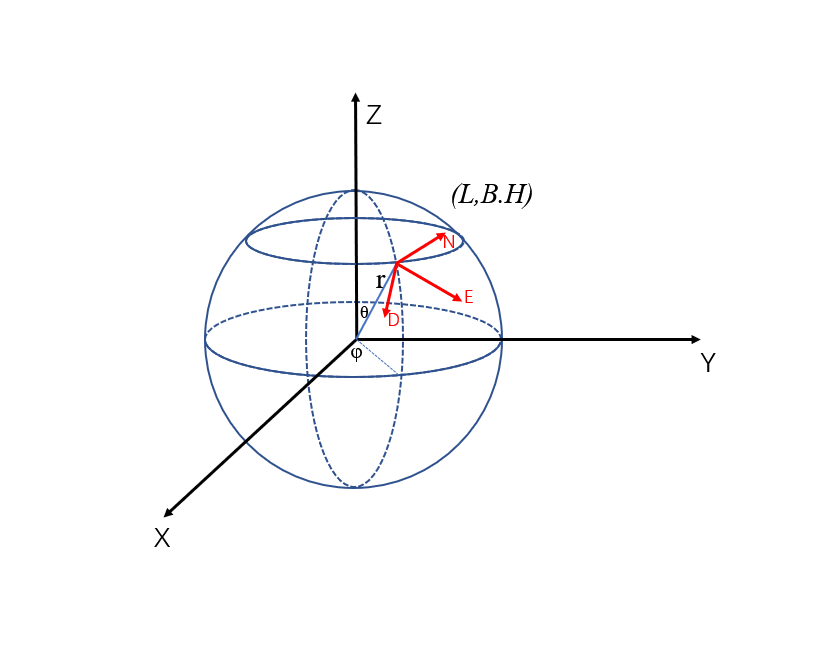
\includegraphics[scale=0.5]{axis.png}
    \caption{各种坐标系关系示意图}
\end{figure}

WGS 84大地坐标系$\longrightarrow$球心坐标系:
WGS84是一种大地坐标系,使用经度、纬度和海拔高度来表示地球上的位置。WGS84的坐标系原点位于地球质心处,因此需要将大地坐标系转换为球心坐标系来进行地球上点的计算。

球心坐标系是一种三维笛卡尔坐标系,它使用X、Y、Z坐标轴表示点在三个方向上的位置。球心坐标系的原点位于地球质心,因此所有地球上的点都可以用X、Y、Z坐标来表示。

转换大地坐标系到球心坐标系的公式如下:
\begin{equation}
    \begin{aligned}
    &X = (N + H) * cosB * cosL \\
    &Y = (N + H) * cosB * sinL\\
    &Z = [N * (1 - e²) + H] * sinB\\
    \end{aligned}
\end{equation}

其中,B是纬度,L是经度,H是海拔高度,N是地球半径在该点的半径,e²是椭球的离心率的平方,其值为0.00669437999014。
X、Y、Z分别表示球心坐标系中点的三个方向上的坐标。
H是点的海拔高度,表示点相对于地球表面的高度。
N是地球半径在该点的半径,表示从地球中心到该点的距离。
e²是椭球的离心率的平方,用于计算N。

球心坐标系$\longrightarrow$站心坐标系NED:
NED坐标系:North-East-Down,简写为NED。
\begin{equation}
    \begin{aligned}
    &N = -sin(B) * cos(L) * X_0 - sin(B) * sin(L) * Y_0 + cos(B) * Z_0\\
    &E = -sin(L) * X_0 + cos(L) * Y_0\\
   &D = -cos(B) * cos(L) * X_0 - cos(B) * sin(L) * Y_0 - sin(B) * Z_0\\
    \end{aligned}
\end{equation}
其中,B是纬度,L是经度,$X_0$,$Y_0$,$Z_0$分别表示球心坐标系原点相对于参考点的位置坐标。

经过坐标系转换的点已经是理想条件下RTK系统所处的站心坐标系下的位置信息,再与RTK中得到的点的roll、yaw、pitch三项结合,就可以作为机器人系统的位姿信息使用,参与后续计算中的位姿变换等。


\subsection{激光里程计和视觉里程计}
激光里程计定位(Laser Odometry and Mapping,LOAM)和视觉里程计定位(Visual Odometry,VO)是两种常用的基于传感器数据的定位方法,它们可以用于机器人、自动驾驶等应用中。
激光里程计定位方法使用激光雷达作为传感器,通过激光点云数据来计算机器人的运动和位置。在LOAM中,激光雷达发射激光束并接收反射回来的光,生成点云数据。然后,通过分析这些点云数据,可以计算出机器人的位置和姿态。
视觉里程计定位方法使用相机作为传感器,通过相机图像来计算机器人的运动和位置。在VO中,通过相邻帧之间的图像差异,来计算机器人的相对运动。然后,通过相机内参和外参等参数,将相对运动转化为机器人在三维空间中的运动。
相较而言,激光里程计定位方法的优点是精度高、鲁棒性强、适用于复杂环境。视觉里程计定位方法的优点是设备便携、成本低、适用于室内场景。然而,视觉里程计定位对光线、噪声等环境条件要求更高,激光里程计定位则对计算资源要求更高。通常对这两者加以结合,扬长避短,获得不错的定位效果。
通常,激光里程计和视觉里程计会应用于SLAM系统中,近些年来,出现了相当一批具有代表性的工作,视觉领域中,\citet{mur2017orb}提出了一种基于特征点的稠密SLAM系统,通过在图像中提取ORB特征点,并使用RANSAC等算法来计算相机运动和场景深度信息。该系统具有实时性、准确性和鲁棒性等优点,在室内和室外场景中都能够进行定位和地图构建。并且于2020年提出了ORB-SLAM2的改进版本,增加了对相机、地图再定位的支持。\citet{qin2018vins}提出了一种基于单目相机和IMU的VIO系统,称为VINS-Mono。该系统采用了一个可扩展的状态估计器,可以实现高精度、低延迟的定位。而在激光领域中,前面提到的\cite{shan2018lego}是一种基于激光雷达的稠密SLAM系统,通过使用分段扫描匹配和点云配准等算法,来计算机器人的运动和位置。该系统具有高精度、实时性和鲁棒性等优点,在大型、复杂环境中进行定位和地图构建。

视觉和激光的融合领域亦有突出的工作,\citet{wisth2021unified}提出了一种基于融合激光雷达、视觉和惯性传感器的紧耦合定位方法,称为LVI-Odometry。在该方法中,激光雷达、视觉和惯性传感器互相协同,实现了高精度的实时定位。LVI-Odometry将SLAM问题转化为多模态地标跟踪问题,通过优化地标的状态估计,从而实现机器人的位姿估计。


\section{运动控制}
移动机器人领域最常用的运动控制方法主要有6种,每一种有具有其独特性质。

PID控制器:PID控制器是一种基于反馈的控制器,可以对机器人的位置、速度、加速度等运动状态进行控制。PID控制器的优点是简单易实现,可以通过调整参数来满足不同的运动要求,但在一些复杂的控制任务中,需要较为复杂的控制算法。

路径追踪控制:路径追踪控制是一种基于轨迹的控制方法,它可以根据预设的轨迹来控制机器人的运动,以达到预期的运动效果。路径追踪控制的优点是可以精确控制机器人的运动轨迹,但需要对机器人和环境进行精确建模。

动力学控制:动力学控制是一种基于物理模型的控制方法,它通过建立机器人的动力学模型,对机器人进行运动控制。动力学控制的优点是可以考虑机器人的动态特性,能够处理高速运动和非线性系统的控制问题,但需要对机器人的动力学进行精确建模。

人工势场控制:人工势场控制是一种基于势场的控制方法,它通过建立机器人和环境的势场,控制机器人沿着势场梯度方向运动。人工势场控制的优点是简单易实现,能够实现障碍物的避障和动态避障,但容易出现局部最小值陷阱问题。

模糊控制:模糊控制是一种基于模糊逻辑的控制方法,它通过将模糊逻辑应用于机器人的控制系统中,对机器人进行运动控制。模糊控制的优点是可以处理模糊和不确定性的问题,但需要进行大量的经验调试。

强化学习:强化学习是一种基于试错学习的控制方法,它通过与环境交互来学习最优的行动策略。强化学习的优点是能够处理复杂的非线性系统和未知环境下的控制问题,但需要大量的训练时间和计算资源。

\section{局部避障}
移动机器人的安全稳定性很大程度上需要靠导航系统的避障功能来保障。通过传感器对周边环境中障碍物的感知,确定自身与障碍物距离,并且通过算法避开障碍物的区域。这种避障是可以轻易做到的,但是移动机器人不仅仅是面临当前避障的考验,还要面临相应的避障之后的移动规划问题。故相应的避障策略必须有所调整。

ORCA(Optimal Reciprocal Collision Avoidance):
是一种局部避障方法,它是一种基于动态几何的方法,通过计算机模拟人类在复杂环境中避免碰撞的行为来实现避障。它主要用于多智能体系统中的避障问题,如机器人团队协作、无人机编队等。

ORCA算法的基本思路是将每个机器人视为圆形,然后利用圆形的运动学约束计算机器人的速度范围,再根据其周围的障碍物信息计算机器人的速度矢量,以避免与周围机器人发生碰撞。ORCA算法的优点是计算简单、易于实现,适用于高密度机器人交通场景。

ORCA算法的缺点是不能处理动态障碍物,即不适用于环境中出现突然障碍物的情况。此外,ORCA算法存在局限性,可能会导致机器人进入局部最小化陷阱(Local Minima Trap)或者被卡在障碍物周围无法移动。因此,在实际应用中,需要根据具体的场景进行优化和改进。

MPC(Model Predictive Control):
也常常运用于移动机器人导航系统的避障功能中,在MPC中,避障问题通常被看作是一种约束条件,通过将避障约束加入到控制器中,来实现机器人的安全移动。在实现中,可以通过在MPC控制器中引入障碍物的状态信息和避障目标函数,以指导机器人的运动轨迹规划。具体来说,MPC避障方法的基本步骤包括:

建立机器人的动力学模型和环境模型,包括机器人的位置、速度、加速度等状态信息,以及环境中的障碍物信息。

利用动力学模型和环境模型,在预测时间窗口内计算机器人的轨迹,以及与障碍物的相对位置。

将避障目标函数引入到MPC控制器中,例如最小化机器人与障碍物的距离,或者最大化机器人可行的运动范围。

在实时控制中,通过调节控制器的参数,来实现机器人的避障和安全移动。

MPC避障方法具有灵活性和可扩展性,适用于不同类型的移动机器人,如无人车、无人机等。同时,MPC避障方法可以考虑到机器人的动态特性和环境的不确定性,具有更好的鲁棒性和性能。